\documentclass[aspectratio=169,10pt]{beamer}

\usepackage[T1]{fontenc}
\usepackage{lmodern}
\usepackage{amsmath,amssymb}
\usepackage{booktabs}
\usepackage{graphicx}
\usepackage{array}
\usepackage{ragged2e}

% Minimal conference palette: dark navy plus one teal accent.
\definecolor{Navy}{HTML}{18334F}
\definecolor{Teal}{HTML}{007C78}
\definecolor{Ink}{HTML}{202830}
\definecolor{Muted}{HTML}{66727D}
\definecolor{Canvas}{HTML}{FCFCFB}
\definecolor{Rule}{HTML}{D9DEE2}
\definecolor{PaleTeal}{HTML}{E8F3F2}

\renewcommand{\familydefault}{\sfdefault}
\setbeamercolor{background canvas}{bg=Canvas}
\setbeamercolor{normal text}{fg=Ink,bg=Canvas}
\setbeamercolor{frametitle}{fg=Navy,bg=Canvas}
\setbeamercolor{structure}{fg=Teal}
\setbeamercolor{alerted text}{fg=Teal}

\setbeamerfont{normal text}{size=\fontsize{11.2}{13.5}}
\setbeamerfont{frametitle}{size=\fontsize{21.5}{24},series=\bfseries}
\setbeamerfont{framesubtitle}{size=\fontsize{9.2}{10.8},series=\bfseries}

\setbeamertemplate{navigation symbols}{}
\setbeamersize{text margin left=0.74cm,text margin right=0.74cm}
\setlength{\leftmargini}{1.05em}
\setlength{\leftmarginii}{1.00em}
\setbeamertemplate{itemize item}{\raise0.20ex\hbox{\color{Teal}\scriptsize$\blacksquare$}}
\setbeamertemplate{itemize subitem}{\raise0.15ex\hbox{\color{Teal}\tiny$\blacktriangleright$}}

\setbeamertemplate{frametitle}{%
  \nointerlineskip
  \begin{beamercolorbox}[wd=\paperwidth,leftskip=0.74cm,rightskip=0.74cm]{frametitle}
    \vspace{0.07cm}
    {\raggedright\usebeamerfont{framesubtitle}\color{Teal}\MakeUppercase{\insertframesubtitle}\strut\par}
    \vspace{-0.02cm}
    {\raggedright\usebeamerfont{frametitle}\insertframetitle\strut\par}
    \vspace{0.06cm}
  \end{beamercolorbox}%
  \hspace{0.74cm}{\color{Rule}\rule{\dimexpr\paperwidth-1.48cm\relax}{0.45pt}}
}

\newif\ifbackup
\backupfalse
\setbeamertemplate{footline}{%
  \ifbackup
  \else
    \leavevmode
    \begin{beamercolorbox}[wd=\paperwidth,ht=0.30cm,dp=0.12cm,leftskip=0.74cm,rightskip=0.74cm]{author in head/foot}
      \fontsize{8.8}{10.2}\selectfont\color{Muted}%
      ELEN90098 \hspace{0.38em}|\hspace{0.38em} Workshop 1: Multi-Armed Bandits
      \hfill\insertframenumber/11
    \end{beamercolorbox}%
  \fi
}

\newcommand{\key}[1]{\textcolor{Teal}{\textbf{#1}}}
\newcommand{\smallnote}[1]{{\fontsize{8.8}{10.6}\selectfont\color{Muted}#1}}
\newcommand{\micro}[1]{{\fontsize{7.8}{9.2}\selectfont\color{Muted}#1}}
\newcommand{\metric}[2]{%
  \begin{minipage}[t]{0.47\linewidth}
    {\fontsize{18}{20}\selectfont\color{Navy}\bfseries #1}\par
    \vspace{0.03cm}{\fontsize{9.2}{11}\selectfont\color{Muted}#2}
  \end{minipage}%
}
\newcommand{\callout}[1]{%
  \begin{beamercolorbox}[wd=\dimexpr\linewidth-0.08cm\relax,sep=0.13cm,leftskip=0.14cm,rightskip=0.14cm]{normal text}
    \raggedright\fontsize{10.2}{12.1}\selectfont\color{Navy}\bfseries #1\par
  \end{beamercolorbox}%
}
\newcommand{\flatbox}[1]{%
  \begin{beamercolorbox}[wd=\linewidth,sep=0.14cm,leftskip=0.16cm,rightskip=0.16cm]{block body}
    \raggedright #1\par
  \end{beamercolorbox}%
}
\setbeamercolor{block body}{bg=PaleTeal,fg=Ink}

\graphicspath{{figures/}}

\begin{document}

\begin{frame}[plain]
  \vspace{0.62cm}
  {\color{Teal}\rule{1.10cm}{2.6pt}}\par
  \vspace{0.38cm}
  {\fontsize{25}{28}\selectfont\bfseries\color{Navy}
    Workshop 1: Multi-Armed Bandits\par}
  \vspace{0.18cm}
  {\fontsize{17}{20}\selectfont\color{Ink}
    Exploration, Regret, and Algorithm Comparison\par}

  \vfill

  \begin{columns}[T,onlytextwidth]
    \begin{column}{0.63\textwidth}
      {\fontsize{12.2}{14.5}\selectfont\bfseries Ray Li \& James Condos}\par
      \vspace{0.12cm}
      {\fontsize{10.2}{12.2}\selectfont\color{Muted}
        ELEN90098 Reinforcement Learning for Engineers\par
        University of Melbourne}
    \end{column}
    \begin{column}{0.34\textwidth}
      \raggedleft
      {\fontsize{9.6}{11.5}\selectfont\color{Muted}
        Workshop oral assessment\par
        10 min presentation + 5 min Q\&A}
    \end{column}
  \end{columns}
  \vspace{0.55cm}
\end{frame}

\begin{frame}{Experimental setup}
  \framesubtitle{EXPERIMENT}
  \vspace{-0.08cm}
  \begin{columns}[T,onlytextwidth]
    \begin{column}{0.52\textwidth}
      \begin{align*}
        k &= 10, & q_*(a) &\sim \mathcal{N}(0,1),\\[-0.05cm]
        R_t\mid A_t=a &\sim \mathcal{N}\!\left(q_*(a),1\right).
      \end{align*}
      \vspace{-0.12cm}
      \flatbox{
        \textbf{Fixed testbed, seed 5.} The optimal arm is
        \(a_*=2\) in Python indexing (the third arm), with
        \(q_*(a_*)=2.4308\).
      }
      \vspace{0.15cm}
      \metric{$T=10^4$}{Q4--Q7 horizon}\hfill
      \metric{$M=300$}{independent reruns}
      \vspace{0.10cm}
      \micro{Q3 growth diagnostics extend to \(T=10^5\) with \(M=500\). The same fixed \(q_*\) is used throughout.}
    \end{column}
    \begin{column}{0.44\textwidth}
      \centering
      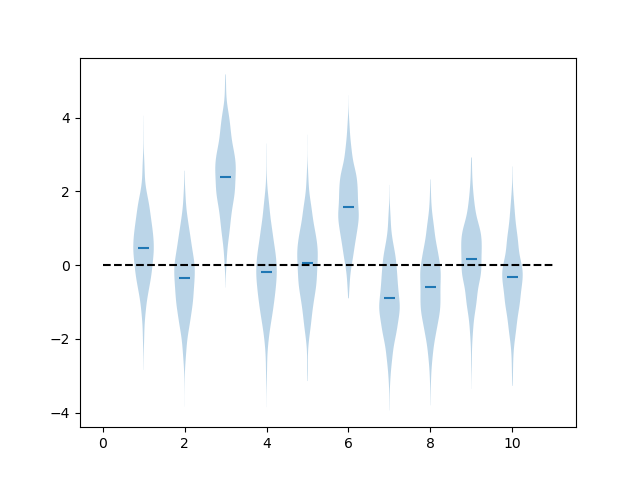
\includegraphics[width=0.92\linewidth]{arms.png}
      \vspace{-0.06cm}
      \smallnote{The simulator knows \(q_*\) only to evaluate pseudo-regret; the agents do not observe it.}
    \end{column}
  \end{columns}
\end{frame}

\begin{frame}{What does sublinear regret mean?}
  \framesubtitle{Q1}
  \vspace{0.08cm}
  \begin{columns}[T,onlytextwidth]
    \begin{column}{0.56\textwidth}
      {\fontsize{11.8}{14.5}\selectfont
      \begin{align*}
        \mathrm{Regret}_T
          &= \mathbb{E}\!\left[\sum_{t=0}^{T-1}
             \bigl(q_*(a_*)-q_*(A_t)\bigr)\right],\\[0.18cm]
        \mathrm{Regret}_T=o(T)
          &\iff \lim_{T\to\infty}\frac{\mathrm{Regret}_T}{T}=0.
      \end{align*}}
      \vspace{0.06cm}
      \callout{Average opportunity loss vanishes, even though cumulative regret may still grow.}
    \end{column}
    \begin{column}{0.39\textwidth}
      \textbf{Why it matters}
      \vspace{0.12cm}
      \begin{itemize}
        \item The policy spends a vanishing fraction of time on inferior arms.
        \item Exploration can continue, but its cumulative cost must grow slower than \(T\).
        \item A straight-looking finite curve is not enough: the growth rate must be tested across horizons.
      \end{itemize}
    \end{column}
  \end{columns}
  \vfill
  \micro{Simulation estimator: \(\widehat R_T=M^{-1}\sum_{r=1}^{M}\sum_{t=0}^{T-1}[q_*(a_*)-q_*(A_t^{(r)})]\).}
\end{frame}

\begin{frame}{How do we test sublinearity numerically?}
  \framesubtitle{Q2}
  \vspace{0.10cm}
  \begin{columns}[T,onlytextwidth]
    \begin{column}{0.31\textwidth}
      \textbf{1. Normalised regret}
      \[
        \widehat\rho_T=\frac{\widehat R_T}{T}
      \]
      \smallnote{Sublinear behaviour requires \(\widehat\rho_T\) to trend toward zero as the horizon grows.}
    \end{column}
    \begin{column}{0.31\textwidth}
      \textbf{2. Incremental slope}
      \[
        \widehat s_{i}=\frac{\widehat R_{T_{i+1}}-\widehat R_{T_i}}
        {T_{i+1}-T_i}
      \]
      \smallnote{A falling late-horizon slope indicates decreasing marginal regret.}
    \end{column}
    \begin{column}{0.31\textwidth}
      \textbf{3. Effective exponent}
      \[
        \widehat\alpha_i=
        \frac{\log \widehat R_{T_{i+1}}-\log \widehat R_{T_i}}
        {\log T_{i+1}-\log T_i}
      \]
      \smallnote{Values below one are consistent with \(\widehat R_T\propto T^{\alpha}\) over that interval.}
    \end{column}
  \end{columns}
  \vspace{0.42cm}
  \flatbox{
    \textbf{Protocol.} Evaluate a common set of horizons
    \(\{10^3,3\!\times\!10^3,10^4,3\!\times\!10^4,10^5\}\), average over 500 reruns, and examine all three diagnostics together.
  }
  \vspace{0.08cm}
  \micro{These are finite-horizon diagnostics. They provide evidence consistent with or against sublinearity; they do not prove an asymptotic theorem.}
\end{frame}

\begin{frame}{Which schedules show sublinear regret?}
  \framesubtitle{Q3 -- EMPIRICAL EVIDENCE}
  \vspace{-0.08cm}
  \begin{columns}[T,onlytextwidth]
    \begin{column}{0.70\textwidth}
      \centering
      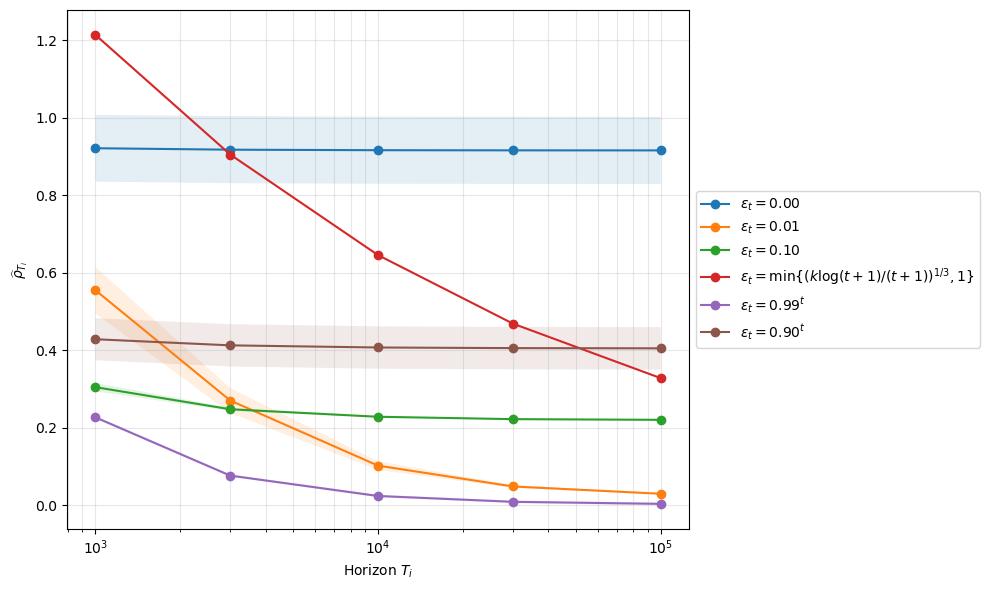
\includegraphics[height=5.20cm,keepaspectratio]{epsilon_multihorizon_normalised_regret.png}
    \end{column}
    \begin{column}{0.27\textwidth}
      \textbf{At \(T=10^5\)}
      \vspace{0.10cm}
      {\fontsize{9.6}{11.3}\selectfont
      \begin{tabular}{@{}lr@{}}
        \toprule
        schedule & \(\widehat\rho_T\)\\
        \midrule
        \(\varepsilon=0\) & 0.9158\\
        \(\varepsilon=0.01\) & 0.0300\\
        \(\varepsilon=0.10\) & 0.2207\\
        polynomial & \textbf{0.3283}\\
        \(0.99^t\) & 0.0040\\
        \(0.90^t\) & 0.4052\\
        \bottomrule
      \end{tabular}}\par
      \vspace{0.13cm}
      \smallnote{Polynomial decay continues to fall with late slope 0.2681. The very small mean for \(0.99^t\) needs a run-level audit.}\par
    \end{column}
  \end{columns}
\end{frame}

\begin{frame}{Why the exploration schedule matters}
  \framesubtitle{Q3 -- INTERPRETATION}
  \vspace{0.12cm}
  \begin{columns}[T,onlytextwidth]
    \begin{column}{0.30\textwidth}
      \textbf{Too little exploration}\par
      \vspace{0.10cm}
      \smallnote{\(\varepsilon=0\) and rapidly decaying \(0.90^t\) can commit early to a wrong arm. Their late slopes remain 0.9157 and 0.4049.}
    \end{column}
    \begin{column}{0.30\textwidth}
      \textbf{Persistent fixed exploration}\par
      \vspace{0.10cm}
      \smallnote{Fixed \(\varepsilon\) keeps sampling inferior arms. The positive regret rate is small for 0.01 but does not vanish in this experiment.}
    \end{column}
    \begin{column}{0.30\textwidth}
      \textbf{Decaying but persistent}\par
      \vspace{0.10cm}
      \smallnote{\(\varepsilon_t=\min\{(k\log(t+1)/(t+1))^{1/3},1\}\) balances continued discovery with decreasing exploration cost.}
    \end{column}
  \end{columns}

  \vspace{0.40cm}
  \flatbox{
    \begin{columns}[T,onlytextwidth]
      \begin{column}{0.23\textwidth}
        {\fontsize{22}{24}\selectfont\bfseries\color{Navy}499/500}\par
        \smallnote{\(0.99^t\) runs with essentially zero late slope}
      \end{column}
      \begin{column}{0.20\textwidth}
        {\fontsize{22}{24}\selectfont\bfseries\color{Teal}1/500}\par
        \smallnote{run with late slope 0.8483}
      \end{column}
      \begin{column}{0.50\textwidth}
        \textbf{A low mean can hide a rare catastrophic run.}\par
        \smallnote{Because \(\sum_t0.99^t<\infty\), exploration eventually becomes negligible; an early wrong commitment can then persist.}
      \end{column}
    \end{columns}
  }
  \vspace{0.05cm}
  \micro{Observed positive-run proportion: 0.002. This is descriptive evidence of a lock-in mechanism, not an estimate of its asymptotic probability.}
\end{frame}

\begin{frame}{UCB arm-value estimation}
  \framesubtitle{Q4}
  \vspace{-0.08cm}
  \centering
  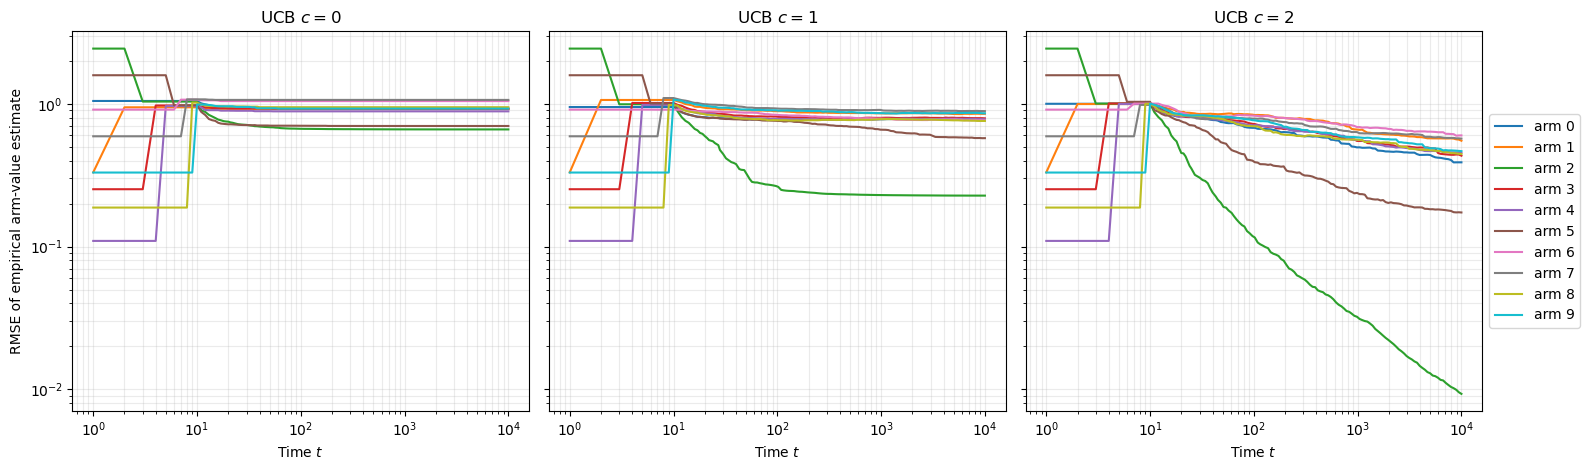
\includegraphics[width=0.85\linewidth]{q4_ucb_arm_value_rmse.png}
  \vspace{-0.01cm}
  \begin{columns}[T,onlytextwidth]
    \begin{column}{0.34\textwidth}
      \textbf{Final mean arm-wise RMSE}\par
      \vspace{0.05cm}
      {\fontsize{8.4}{9.8}\selectfont
      \begin{tabular}{@{}cc@{}}
        \toprule
        UCB \(c\) & mean RMSE\\
        \midrule
        0 & 0.8981\\
        1 & 0.7254\\
        2 & \textbf{0.4090}\\
        \bottomrule
      \end{tabular}}
    \end{column}
    \begin{column}{0.61\textwidth}
      \smallnote{Per arm, \(\mathrm{RMSE}_T(a)=\sqrt{M^{-1}\sum_r(Q_T^{(r)}(a)-q_*(a))^2}\); the table averages this over ten arms.}\par
      \vspace{0.06cm}
      \smallnote{\textbf{Result:} larger \(c\) estimates all arms better. This differs from minimising regret.}
    \end{column}
  \end{columns}
\end{frame}

\begin{frame}{UCB versus epsilon-greedy regret}
  \framesubtitle{Q5}
  \vspace{-0.07cm}
  \begin{columns}[T,onlytextwidth]
    \begin{column}{0.68\textwidth}
      \centering
      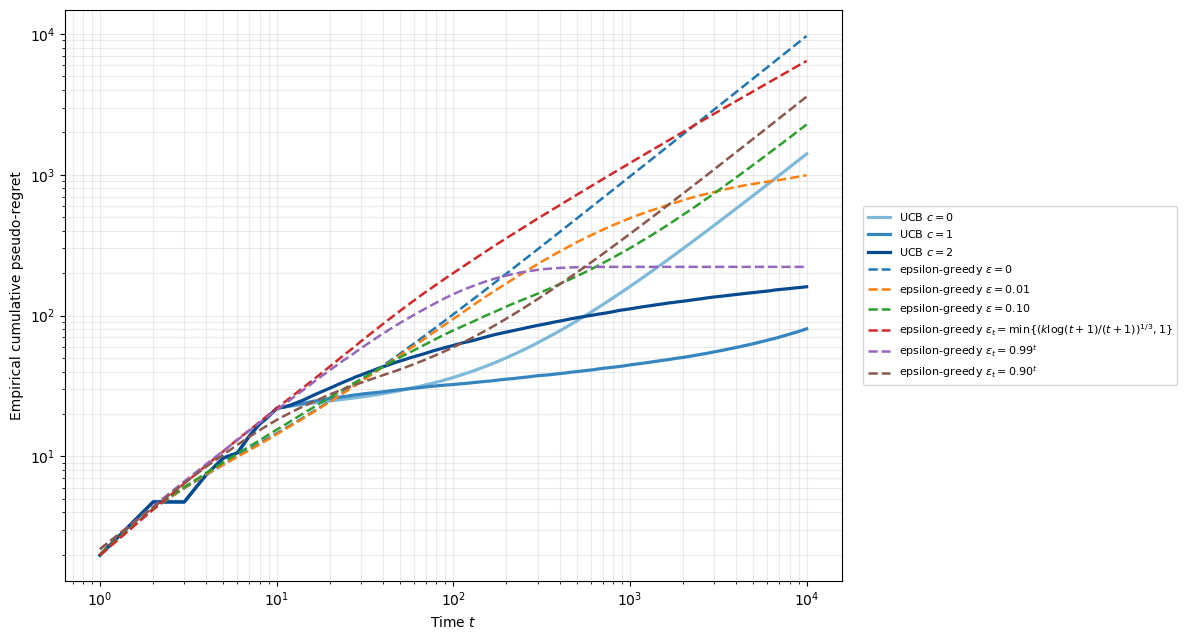
\includegraphics[height=4.70cm,keepaspectratio]{q5_ucb_vs_epsilon_regret.png}
    \end{column}
    \begin{column}{0.29\textwidth}
      \textbf{Regret at \(T=10^4\)}
      \vspace{0.08cm}
      {\fontsize{9.5}{11.2}\selectfont
      \begin{tabular}{@{}lr@{}}
        \toprule
        policy & \(\widehat R_T\)\\
        \midrule
        UCB \(c=1\) & \textbf{80.58}\\
        UCB \(c=2\) & 160.29\\
        \(\varepsilon_t=0.99^t\) & 221.98\\
        \(\varepsilon=0.01\) & 994.19\\
        \bottomrule
      \end{tabular}}\par
      \vspace{0.17cm}
      \callout{Lowest regret: UCB \(c=1\). Lowest RMSE: UCB \(c=2\).}\par
      \vspace{0.07cm}
      \micro{Index: \(Q_t(a)+c\sqrt{\log(t+1)/N_t(a)}\).}
    \end{column}
  \end{columns}
\end{frame}

\begin{frame}{Gradient bandit versus UCB}
  \framesubtitle{Q6}
  \vspace{-0.07cm}
  \begin{columns}[T,onlytextwidth]
    \begin{column}{0.68\textwidth}
      \centering
      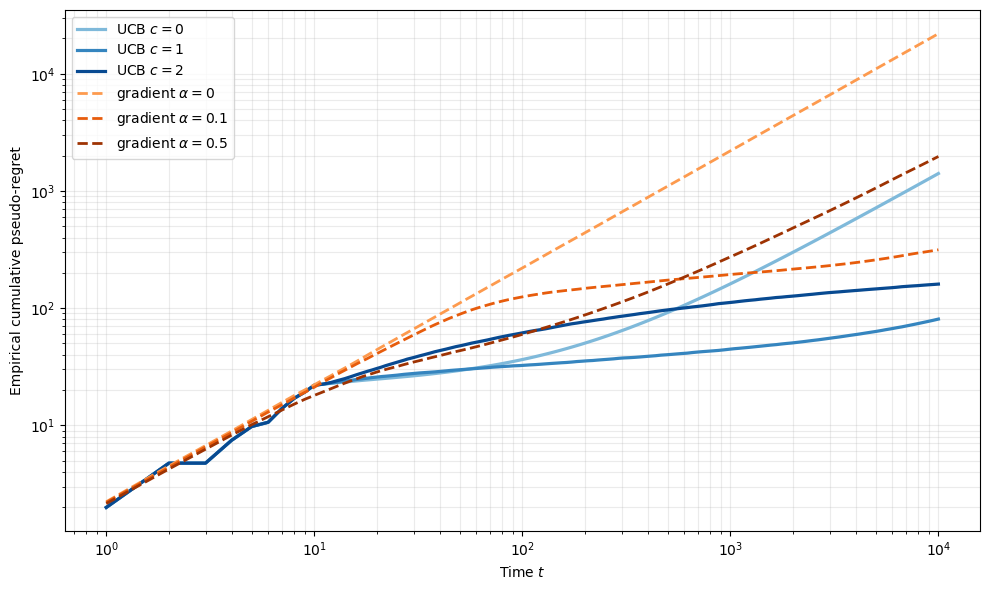
\includegraphics[height=4.70cm,keepaspectratio]{q6_gradient_vs_ucb_regret.png}
    \end{column}
    \begin{column}{0.29\textwidth}
      \textbf{Regret at \(T=10^4\)}
      \vspace{0.08cm}
      {\fontsize{9.3}{11.0}\selectfont
      \begin{tabular}{@{}lr@{}}
        \toprule
        policy & \(\widehat R_T\)\\
        \midrule
        UCB \(c=1\) & \textbf{80.58}\\
        UCB \(c=2\) & 160.29\\
        Grad. \(\alpha=0.1\) & 314.58\\
        Grad. \(\alpha=0.5\) & 1968.16\\
        UCB \(c=0\) & 1408.07\\
        \bottomrule
      \end{tabular}}\par
      \vspace{0.12cm}
      \flatbox{{\fontsize{14.5}{17}\selectfont\bfseries\color{Navy}3.90\(\times\) more regret}\par
      \micro{Best gradient versus UCB \(c=1\), on this experiment.}}
    \end{column}
  \end{columns}
\end{frame}

\begin{frame}{Gradient step-size sensitivity}
  \framesubtitle{Q7}
  \vspace{-0.08cm}
  \begin{columns}[T,onlytextwidth]
    \begin{column}{0.56\textwidth}
      \centering
      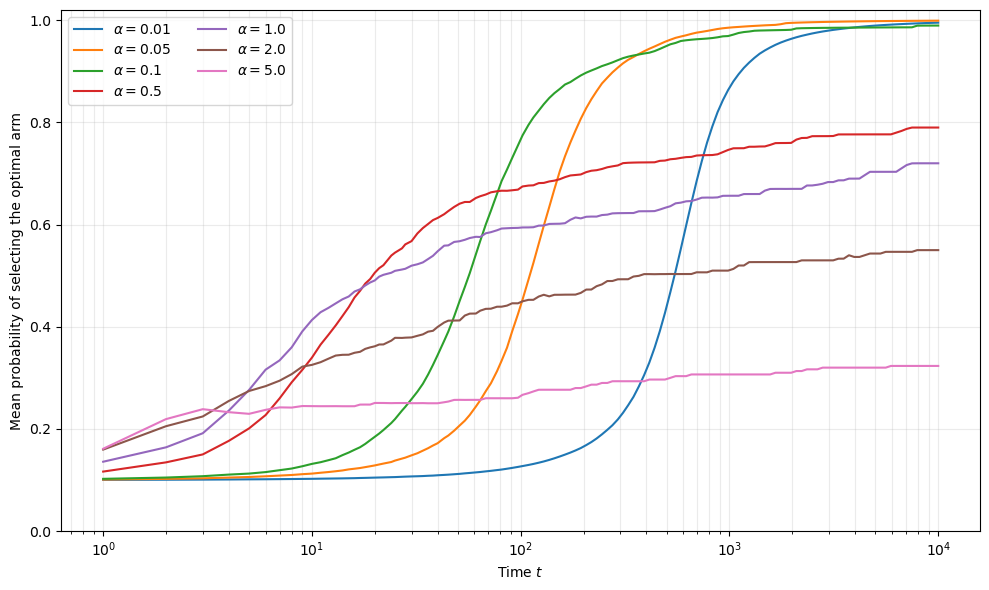
\includegraphics[height=4.25cm,keepaspectratio]{q7_gradient_alpha_sensitivity.png}
    \end{column}
    \begin{column}{0.41\textwidth}
      \textbf{Final performance at \(T=10^4\)}
      \vspace{0.06cm}
      {\fontsize{8.6}{9.8}\selectfont
      \begin{tabular}{@{}rrr@{}}
        \toprule
        \(\alpha\) & mean \(P_T(a_*)\) & \(\widehat R_T\)\\
        \midrule
        0.01 & 0.9952 & 1542.45\\
        0.05 & \textbf{0.9991} & 357.39\\
        0.10 & 0.9896 & \textbf{314.58}\\
        0.50 & 0.7899 & 1968.16\\
        2.00 & 0.5500 & 5358.04\\
        5.00 & 0.3233 & 11148.71\\
        \bottomrule
      \end{tabular}}
      \vspace{0.03cm}
      \flatbox{{\fontsize{9.5}{11.1}\selectfont At \(\alpha=5\): 32.33\% of runs end above 0.99, 67.67\% below 0.01, and none in between.}}\par
      \vspace{-0.01cm}\micro{Our results do not support optimal-arm convergence for arbitrary \(\alpha>0\).}
    \end{column}
  \end{columns}
\end{frame}

\begin{frame}{Conclusions and questions}
  \framesubtitle{Q1--Q7 | SUMMARY}
  \vspace{0.08cm}
  \begin{columns}[T,onlytextwidth]
    \begin{column}{0.65\textwidth}
      \begin{enumerate}
        \item \textbf{Q1--Q2:} sublinear regret means vanishing regret per step; credible finite-horizon evidence needs several complementary diagnostics.
        \item \textbf{Q3:} polynomially decaying exploration gives the clearest sublinear trend; a low average can conceal rare lock-in.
        \item \textbf{Q4--Q5:} UCB \(c=2\) estimates arm values best, while UCB \(c=1\) achieves the lowest regret.
        \item \textbf{Q6--Q7:} gradient bandit works well only in a moderate step-size range; aggressive updates can create bimodal outcomes.
      \end{enumerate}
      \vspace{0.20cm}
      \smallnote{All reported comparisons use the same fixed ten-arm Gaussian testbed and notebook protocols. Claims are empirical unless stated otherwise.}
    \end{column}
    \begin{column}{0.31\textwidth}
      \centering
      \vspace{0.42cm}
      {\color{Teal}\rule{0.82cm}{2.6pt}}\par
      \vspace{0.24cm}
      {\fontsize{25}{28}\selectfont\bfseries\color{Navy}Questions?}\par
      \vspace{0.18cm}
      {\fontsize{10.2}{12.4}\selectfont\color{Muted}5-minute discussion}
    \end{column}
  \end{columns}
\end{frame}


\backuptrue
\begin{frame}{Additional epsilon-greedy diagnostics}
  \framesubtitle{BACKUP A1 -- Q2/Q3}
  \vspace{-0.08cm}
  \centering
  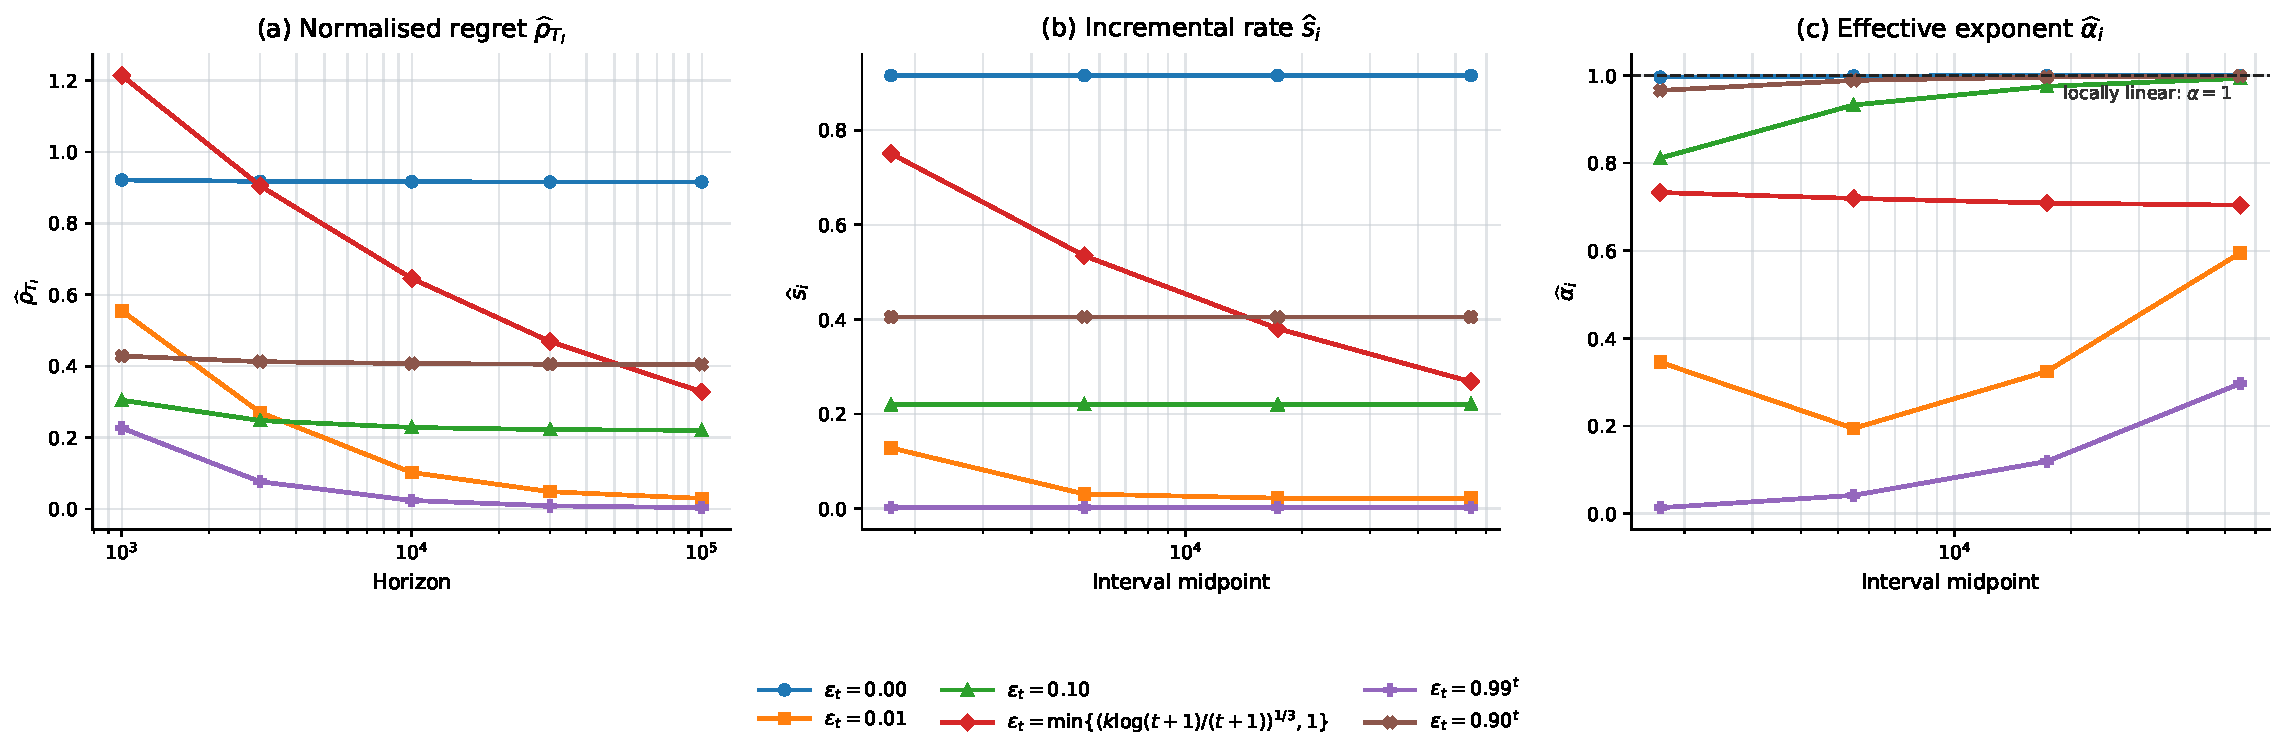
\includegraphics[width=0.99\linewidth]{q3_epsilon_diagnostics_1x3.pdf}
  \vspace{0.02cm}
  \smallnote{The three diagnostics support the same qualitative interpretation; \(\widehat{\alpha}_i\) is supplementary, while \(\widehat{\rho}_{T_i}\) and \(\widehat{s}_i\) are the primary numerical tests.}
\end{frame}

\begin{frame}{Rare-failure audit for $\varepsilon_t=0.99^t$}
  \framesubtitle{BACKUP A2 -- Q3}
  \vspace{0.12cm}
  \begin{columns}[T,onlytextwidth]
    \begin{column}{0.47\textwidth}
      \textbf{Run-level result, \(30{,}000\) to \(100{,}000\)}\par
      \vspace{0.18cm}
      \metric{499}{near-zero-slope runs}\hfill
      \metric{1}{run at slope 0.84829}
      \vspace{0.30cm}
      \begin{tabular}{@{}lr@{}}
        \toprule
        statistic & value\\
        \midrule
        mean late slope & 0.001697\\
        positive-run fraction & 0.002\\
        positive-run slope & 0.84829\\
        \bottomrule
      \end{tabular}
    \end{column}
    \begin{column}{0.48\textwidth}
      \textbf{Mechanism}\par
      \[
        \sum_{t=0}^{\infty}0.99^t = 100 < \infty.
      \]
      \begin{itemize}
        \item Only a finite expected amount of random exploration is scheduled.
        \item Most runs identify the optimal arm before exploration disappears.
        \item A rare early error can survive and then accumulate near-linear regret.
      \end{itemize}
    \end{column}
  \end{columns}
\end{frame}

\begin{frame}{UCB arm-level estimates at T = 10,000}
  \framesubtitle{BACKUP A3 -- Q4}
  \vspace{0.04cm}
  \begin{columns}[T,onlytextwidth]
    \begin{column}{0.61\textwidth}
      {\fontsize{8.6}{10.3}\selectfont
      \begin{tabular}{@{}rrrr@{}}
        \toprule
        arm & \(q_*(a)\) & mean \(Q_T(a)\), \(c=2\) & mean \(N_T(a)\)\\
        \midrule
        0 &  0.441 &  0.316 & 9.3\\
        1 & -0.331 & -0.459 & 5.3\\
        2 &  2.431 &  2.430 & 9900.0\\
        3 & -0.252 & -0.321 & 5.7\\
        4 &  0.110 & -0.004 & 7.2\\
        5 &  1.582 &  1.526 & 44.0\\
        6 & -0.909 & -1.058 & 3.8\\
        7 & -0.592 & -0.755 & 4.4\\
        8 &  0.188 &  0.090 & 7.6\\
        9 & -0.330 & -0.423 & 5.3\\
        \bottomrule
      \end{tabular}}
    \end{column}
    \begin{column}{0.34\textwidth}
      \textbf{Mean arm-wise RMSE}
      \vspace{0.12cm}
      \begin{tabular}{@{}cc@{}}
        \toprule
        \(c\) & RMSE\\
        \midrule
        0 & 0.8981\\
        1 & 0.7254\\
        2 & \textbf{0.4090}\\
        \bottomrule
      \end{tabular}\par
      \vspace{0.24cm}
      \smallnote{Even \(c=2\) allocates almost all pulls to the best arm. Its extra exploration primarily improves estimates of the remaining arms.}
    \end{column}
  \end{columns}
\end{frame}

\begin{frame}{Full gradient step-size sweep}
  \framesubtitle{BACKUP A4 -- Q7}
  \vspace{0.04cm}
  \begin{columns}[T,onlytextwidth]
    \begin{column}{0.62\textwidth}
      {\fontsize{9.1}{10.9}\selectfont
      \begin{tabular}{@{}rrrrr@{}}
        \toprule
        \(\alpha\) & mean \(P_T(a_*)\) & regret & \(P_T>0.99\) & \(P_T<0.01\)\\
        \midrule
        0.01 & 0.9952 & 1542.45 & 1.0000 & 0.0000\\
        0.05 & 0.9991 & 357.39 & 1.0000 & 0.0000\\
        0.10 & 0.9896 & 314.58 & 0.9900 & 0.0100\\
        0.50 & 0.7899 & 1968.16 & 0.7900 & 0.2100\\
        1.00 & 0.7200 & 2765.23 & 0.7200 & 0.2800\\
        2.00 & 0.5500 & 5358.04 & 0.5500 & 0.4500\\
        5.00 & 0.3233 & 11148.71 & 0.3233 & 0.6767\\
        \bottomrule
      \end{tabular}}
    \end{column}
    \begin{column}{0.33\textwidth}
      \textbf{Why ``between'' is zero}\par
      \vspace{0.12cm}
      \smallnote{The final-policy distribution is almost binary: each run ends either strongly on the optimal arm or strongly on another arm. Therefore}
      \[
        \Pr(0.01\le P_T(a_*)\le0.99)=0
      \]
      \smallnote{for every tested \(\alpha\). This column measures concentration, not statistical uncertainty.}
    \end{column}
  \end{columns}
\end{frame}

\begin{frame}{Algorithms used in the comparison}
  \framesubtitle{BACKUP A5 -- METHODS}
  \vspace{0.08cm}
  \begin{columns}[T,onlytextwidth]
    \begin{column}{0.38\textwidth}
      \textbf{Epsilon-greedy}\par
      \vspace{0.06cm}
      \smallnote{With probability \(1-\varepsilon_t\), select a greedy action; otherwise sample uniformly. Values use sample-average updates.}
      \vspace{0.30cm}

      \textbf{Upper confidence bound}\par
      \vspace{0.04cm}
      {\fontsize{8.8}{10.6}\selectfont
      \[
        A_t=\arg\max_a\left[
          Q_t(a)+c\sqrt{\frac{\log(t+1)}{N_t(a)}}
        \right].
      \]}
      \smallnote{The bonus favours actions with uncertain value estimates.}
    \end{column}
    \begin{column}{0.57\textwidth}
      \textbf{Gradient bandit}\par
      \vspace{0.05cm}
      {\fontsize{9.2}{11.1}\selectfont
      \[
        \pi_t(a)=
        \frac{\exp\!\left(H_t(a)-\max_b H_t(b)\right)}
        {\sum_b\exp\!\left(H_t(b)-\max_j H_t(j)\right)}.
      \]
      \[
        \Delta H_t(a)=\alpha(R_t-\bar R_t)
        \left(\mathbf{1}_{a=A_t}-\pi_t(a)\right).
      \]}
      \smallnote{Preferences are updated by reward advantage relative to the running-average baseline. The shifted softmax is numerically stable.}
    \end{column}
  \end{columns}
\end{frame}


\end{document}
